%%%%%%%%%%%%%%%%%%%%%%%%%%%
%
% $Autor: Wings $
% $Datum: 2020-07-24 09:05:07Z $
% $Pfad: GDV/Vortraege/latex - Ausarbeitung/Kapitel/MapleDateien.tex $
% $Version: 4732 $
%
%%%%%%%%%%%%%%%%%%%%%%%%%%%
%\VERSION{$ $Pfad: GDV/Vortraege/latex - Ausarbeitung/Kapitel/MapleDateien.tex $ $}{$ $Version: 4732 $ $}



\chapter{Data Mining}

\section{Stage Data Mining}



Here we, presents the data-driven methodologies employed in the hurricane intensity prediction system, integrating principles of data mining with time-series forecasting models. The primary goal is to estimate future wind speeds of hurricanes using historical data to improve early warning systems and disaster preparedness. The system first leverages data mining techniques to extract meaningful patterns from spatiotemporal hurricane datasets. For example, Dong and Pi (2013) developed a trajectory-based hurricane prediction method using frequent pattern mining and rule generation, which demonstrated substantial accuracy improvements by learning from historical movement patterns \cite{dong2013htpdm}. Building upon such mined insights, the forecasting framework implements two core predictive models: ARIMA and LSTM. The AutoRegressive Integrated Moving Average (ARIMA) model is well-suited for capturing linear dependencies and trend components in short-term time-series data. Zhang et al. (2022) introduced a variant called BHT-ARIMA, optimized for tropical cyclone intensity prediction within 6 to 12 hours, showing superior performance in short-range forecasting scenarios \cite{zhang2022bhtarima}. On the other hand, Long Short-Term Memory (LSTM) neural networks are capable of modeling long-term dependencies and non-linear dynamics in time series. Li et al. (2020) proposed a global LSTM-based framework for rapid intensification forecasting, demonstrating improved prediction accuracy over classical methods across several hurricane basins \cite{li2020lstmrapid}. These models are integrated into the system using a modular architecture comprising scripts such as


The discussion includes the theoretical foundations, algorithmic relevance to the problem domain, computational considerations, input/output structure, hyperparameter details, and alignment with project implementation scripts (\texttt{app.py}, \texttt{developer.py}, \texttt{model\_utils.py}, \texttt{train\_models.ipynb}).

\subsection{ARIMA Model}

The ARIMA model combines autoregressive (AR), differencing (I), and moving average (MA) components to model time series data with strong short-term dependencies. It is particularly effective when the dataset exhibits trend and seasonality after appropriate transformations. ARIMA’s statistical interpretability and minimal computational overhead make it well-suited for near-future hurricane wind-speed forecasting.

Recent research by Zhang et al. (2022) proposed a short-term cyclone intensity forecasting method based on BHT-ARIMA and demonstrated significant improvements in forecast accuracy within 6–12 hours of prediction \cite{zhang2022bhtarima}.

\subsection{LSTM Model}

LSTM, a variant of Recurrent Neural Networks (RNNs), addresses the vanishing gradient problem and is capable of modeling long-term dependencies in sequential data. It has become a standard deep learning approach in temporal forecasting tasks. In the context of hurricanes, LSTM enables the model to learn complex, non-linear temporal relationships that traditional statistical models often fail to capture.

Li et al. (2020) developed a global LSTM-based framework for predicting rapid intensification of hurricanes and showed that deep learning significantly improves prediction skill over classical methods \cite{li2020lstmrapid}.

\subsection{Implementation Alignment}

The methodologies are implemented using the following system components:
\begin{itemize}
	\item \texttt{app.py}: Provides an intuitive Streamlit-based graphical interface for data upload and forecast visualization.
	\item \texttt{developer.py}: Defines model hyperparameters and configures whether ARIMA or LSTM is used.
	\item \texttt{model\_utils.py}: Includes common utilities such as data normalization, error metric calculation (RMSE, MAE), and data splitting.
	\item \texttt{train\_models.ipynb}: An exploratory Jupyter notebook used during model development and tuning phases.
\end{itemize}

These components collectively ensure seamless integration of the forecasting logic into an accessible and user-friendly application.



\subsection{Algorithm Description}

\subsubsection{ARIMA (AutoRegressive Integrated Moving Average)}

\textbf{Overview}: ARIMA is a classical statistical framework for time-series forecasting that combines three components: autoregressive (AR), differencing (I), and moving average (MA) \cite{BoxEtAl2015}. The AR part models dependencies on past values (order $p$), the differencing component ($d$) ensures stationarity by removing trends, and the MA part models the dependency on past forecast errors (order $q$).

\begin{itemize}
	\item \textbf{Implementation}: In \texttt{model\_utils.py}, the \texttt{train\_arima\_model} function uses the \texttt{statsmodels} library to fit an ARIMA($p,d,q$) model with parameters configurable in \texttt{config2.json}. The trained model is saved as \texttt{arima\_model.pkl} and loaded in \texttt{app.py} to forecast up to 30 time steps ahead.
	\item \textbf{Technical Details}: ARIMA assumes stationarity, achieved via differencing. The training notebook \texttt{train\_models.ipynb} displays warnings if the differencing order is insufficient, emphasizing the need to tune $d$. ARIMA offers computational efficiency suitable for quick forecasting.
\end{itemize}

\subsubsection{LSTM (Long Short-Term Memory)}

\textbf{Overview}: LSTM is a specialized recurrent neural network architecture capable of capturing long-term dependencies in sequential data through gated memory cells, addressing the vanishing gradient problem typical of standard RNNs \cite{HochreiterSchmidhuber1997}.

\begin{itemize}
	\item \textbf{Implementation}: In \texttt{developer.py} and \texttt{train\_models.ipynb}, a two-layer LSTM network with 50 units per layer followed by a dense output layer is constructed using TensorFlow/Keras. Input sequences of wind speeds (default length 10, per \texttt{config2.json}) are scaled with \texttt{MinMaxScaler}. The trained model and scaler are saved as \texttt{lstm\_model.h5} and \texttt{lstm\_scaler.pkl} for use in \texttt{app.py}.
	\item \textbf{Technical Details}: LSTM captures non-linear temporal patterns, suited to chaotic systems like hurricanes. Training uses backpropagation through time with the Adam optimizer and mean squared error (MSE) loss, monitored in \texttt{developer.py}.
\end{itemize}

\subsection{Applications}

\subsubsection{ARIMA Applications}

\begin{itemize}
	\item \textbf{General}: ARIMA is widely used in financial forecasting (e.g., stock prices), macroeconomic indicators (e.g., GDP, inflation), and environmental modeling (e.g., temperature trends).
	\item \textbf{Project-Specific}: ARIMA forecasts hurricane wind speeds for up to 30 days in \texttt{app.py}, aiding proactive disaster response. Time-series forecasting is fundamental in meteorology \cite{Emanuel2005}.
	\item \textbf{Suitability}: ARIMA works best on stationary or near-stationary datasets with linear dependencies, as ensured by preprocessing steps in \texttt{model\_utils.py}. Its interpretability helps validate forecast outcomes.
\end{itemize}

\subsubsection{LSTM Applications}

\begin{itemize}
	\item \textbf{General}: LSTM excels in modeling complex sequential data in NLP, speech recognition, and time-series forecasting in domains such as energy and weather.
	\item \textbf{Project-Specific}: LSTM captures the nonlinear and chaotic dynamics of hurricane wind speeds using historical sequences, providing flexible sequence-length configuration via \texttt{developer.py}.
	\item \textbf{Suitability}: Its ability to learn long-term dependencies and nonlinear relationships makes LSTM well-suited to forecasting hurricane intensities.
\end{itemize}

\textbf{Technical Insight}: The dual-model strategy (\texttt{config2.json}) balances ARIMA’s simplicity and LSTM’s modeling power, allowing tailored forecasting strategies implemented in \texttt{developer.py}.

\subsection{Relevance}

\textbf{Problem Context}: Accurate wind speed forecasting is essential for disaster preparedness in hurricane-prone regions. The models must handle temporal patterns effectively to predict storm severity.

\begin{itemize}
	\item \textbf{ARIMA}: Appropriate for stationary, linear data after preprocessing (missing value imputation, sorting) as in \texttt{app.py}. Its speed enables real-time forecasting \cite{HyndmanAthanasopoulos2021}.
	\item \textbf{LSTM}: Addresses ARIMA’s limitations by modeling nonlinear, chaotic behavior with flexible sequence lengths.
	\item \textbf{Synergy}: Ability to switch between ARIMA and LSTM allows robustness across diverse hurricane profiles.
\end{itemize}

\textbf{Technical Insight}: Input validation (e.g., minimum data points) in \texttt{app.py} ensures reliable forecasting. ARIMA offers interpretable forecasts, while LSTM enhances accuracy for complex patterns.

\subsection{Hyperparameters}

\textbf{Definition}: Hyperparameters control model behavior and are tuned before training to balance accuracy, overfitting, and computation.

\subsubsection{ARIMA Hyperparameters}

\begin{itemize}
	\item $p$: AR order (default 2).
	\item $d$: Differencing order for stationarity (default 1).
	\item $q$: MA order (default 2).
	\item \textbf{Configuration}: Adjustable via \texttt{developer.py} interface with limits ($p, q \leq 5$, $d \leq 2$) enforced in \texttt{train\_models.ipynb} to prevent overfitting.
	\item \textbf{Impact}: Larger $p$ or $q$ increases complexity; $d$ affects stationarity and forecast quality.
\end{itemize}

\subsubsection{LSTM Hyperparameters}

\begin{itemize}
	\item \textbf{Epochs}: Number of training iterations (default 10).
	\item \textbf{Batch Size}: Samples per update (default 32).
	\item \textbf{Sequence Length}: Past steps used for prediction (default 10).
	\item \textbf{Units}: LSTM units per layer (fixed 50).
	\item \textbf{Learning Rate}: Optimizer step size (default 0.001).
	\item \textbf{Configuration}: Limited adjustment in \texttt{developer.py} to ensure ease of use.
	\item \textbf{Impact}: More epochs/units improve learning but risk overfitting; sequence length affects temporal context captured.
\end{itemize}

\textbf{Technical Insight}: Modular design supports iterative hyperparameter tuning.

\subsection{Data and Computation Requirements}

\subsubsection{Data Requirements}

\begin{itemize}
	\item \textbf{Input}: Historical wind speed time series with timestamps, cleaned via imputation and sorting in \texttt{app.py}.
	\item \textbf{Minimum Data}: ARIMA requires at least 10 points; LSTM needs sequence length + 1 points.
	\item \textbf{Data Quality}: Stationary and clean data is critical for ARIMA; LSTM is more tolerant of noise but requires scaled inputs.
\end{itemize}
\begin{center}
	\resizebox{!}{10cm}{ % fix height to 10cm
		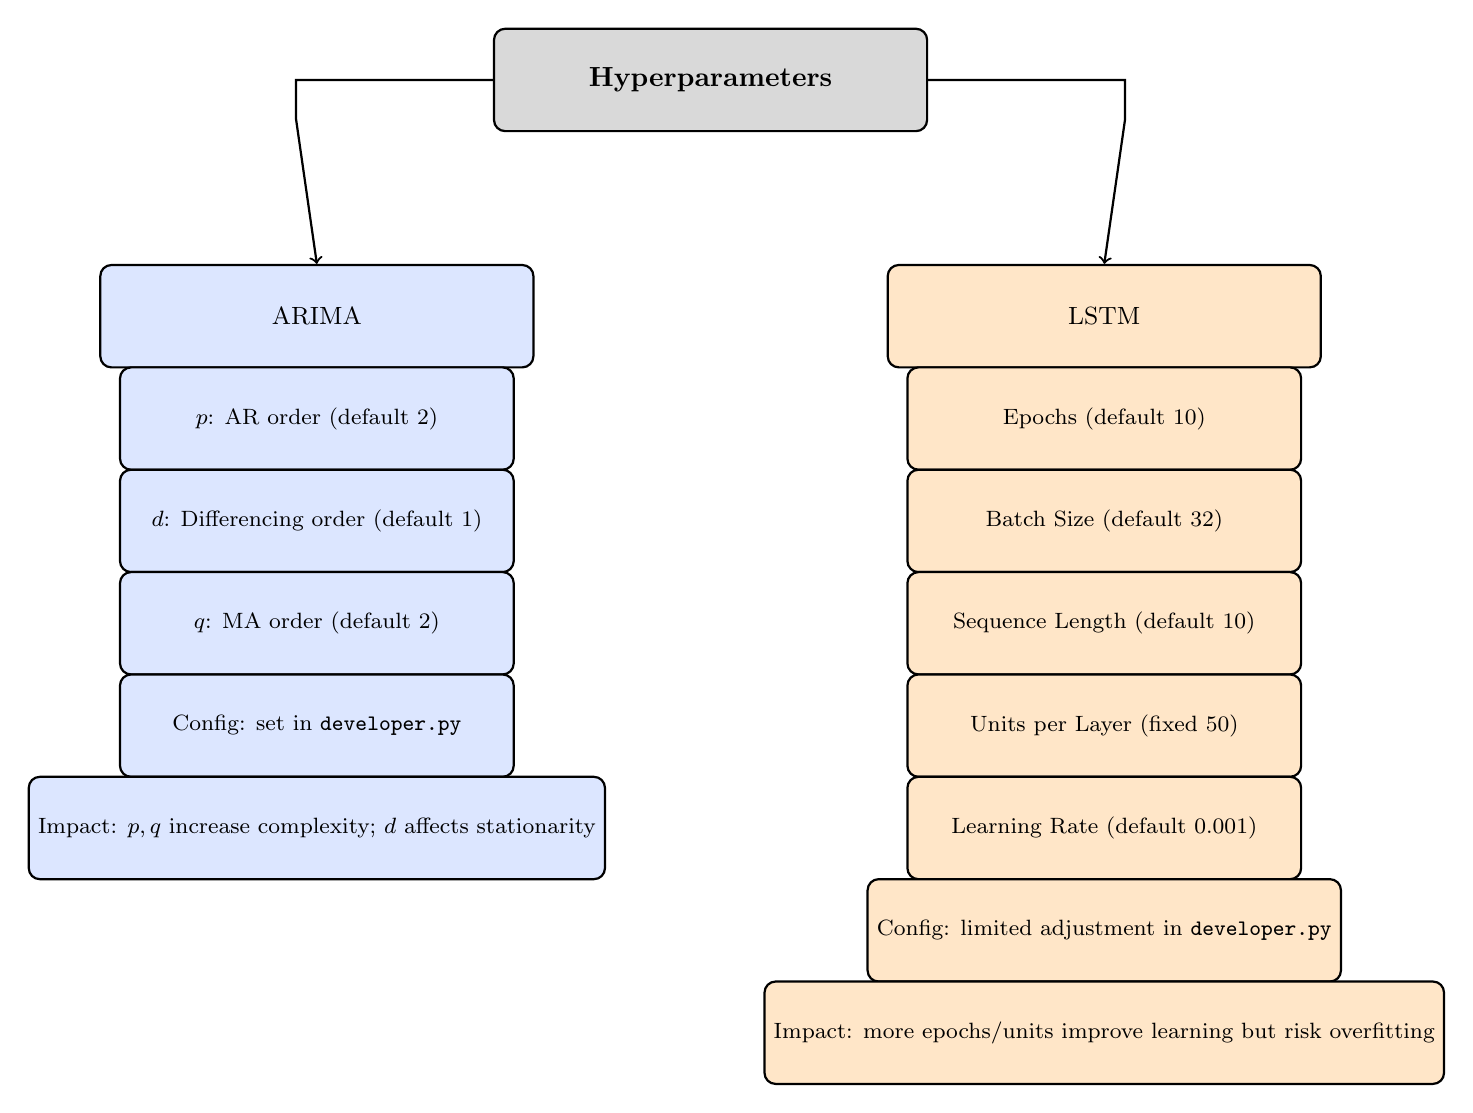
\begin{tikzpicture}[font=\small]
			
			% Styles
			\tikzset{
				box/.style={
					rectangle, draw=black, thick,
					minimum width=5.5cm, minimum height=1.3cm,
					text centered,
					rounded corners,
					fill=#1,
				},
				arrow/.style={
					thick, ->,
				}
			}
			
			% Colors
			\definecolor{mybluebg}{RGB}{220,230,255}
			\definecolor{myorangebg}{RGB}{255,230,200}
			
			% Title box
			\node[box=gray!30, font=\bfseries] (hyper) at (0,0) {Hyperparameters};
			
			% ARIMA main box (left)
			\node[box=mybluebg] (arima) at (-5,-3) {ARIMA};
			
			% ARIMA details stacked vertically below ARIMA box, more spacing now
			\node[box=mybluebg, minimum width=5cm, font=\footnotesize] (p) at (-5,-4.3) {$p$: AR order (default 2)};
			\node[box=mybluebg, minimum width=5cm, font=\footnotesize] (d) at (-5,-5.6) {$d$: Differencing order (default 1)};
			\node[box=mybluebg, minimum width=5cm, font=\footnotesize] (q) at (-5,-6.9) {$q$: MA order (default 2)};
			\node[box=mybluebg, minimum width=5cm, font=\footnotesize] (configA) at (-5,-8.2) {Config: set in \texttt{developer.py}};
			\node[box=mybluebg, minimum width=5cm, font=\footnotesize] (impactA) at (-5,-9.5) {Impact: $p,q$ increase complexity; $d$ affects stationarity};
			
			% LSTM main box (right)
			\node[box=myorangebg] (lstm) at (5,-3) {LSTM};
			
			% LSTM details stacked vertically below LSTM box, more spacing
			\node[box=myorangebg, minimum width=5cm, font=\footnotesize] (epochs) at (5,-4.3) {Epochs (default 10)};
			\node[box=myorangebg, minimum width=5cm, font=\footnotesize] (batch) at (5,-5.6) {Batch Size (default 32)};
			\node[box=myorangebg, minimum width=5cm, font=\footnotesize] (seq) at (5,-6.9) {Sequence Length (default 10)};
			\node[box=myorangebg, minimum width=5cm, font=\footnotesize] (units) at (5,-8.2) {Units per Layer (fixed 50)};
			\node[box=myorangebg, minimum width=5cm, font=\footnotesize] (lr) at (5,-9.5) {Learning Rate (default 0.001)};
			\node[box=myorangebg, minimum width=5cm, font=\footnotesize] (configL) at (5,-10.8) {Config: limited adjustment in \texttt{developer.py}};
			\node[box=myorangebg, minimum width=5cm, font=\footnotesize] (impactL) at (5,-12.1) {Impact: more epochs/units improve learning but risk overfitting};
			
			% Arrows from hyperparameters to ARIMA and LSTM (horizontal then vertical down)
			\draw[arrow] (hyper.west) -- ++(-2.5,0) -- ++(0,-0.5) -- (arima.north);
			\draw[arrow] (hyper.east) -- ++(2.5,0) -- ++(0,-0.5) -- (lstm.north);
			
		\end{tikzpicture}
	}
\end{center}






\subsubsection{Computation Requirements}

\begin{itemize}
	\item \textbf{Hardware}: ARIMA runs efficiently on CPU; LSTM benefits from GPU but can run on CPU with longer training.
	\item \textbf{Software}: Python 3.x, with \texttt{statsmodels}, \texttt{TensorFlow/Keras}, \texttt{scikit-learn}, \texttt{numpy}, and \texttt{pandas}.
	\item \textbf{Runtime}: ARIMA training takes seconds to minutes; LSTM can take minutes to hours depending on data and epochs.
\end{itemize}

\subsection{Input and Output}
\subsection{Input}
% Overview of inputs
\textbf{Overview}: Inputs are the preprocessed data fed into the algorithms.

% ARIMA input
\subsubsection{ARIMA Input}
\begin{itemize}
	\item \textbf{Format}: A univariate time-series of wind speeds, sorted chronologically.
	\item \textbf{Preprocessing}:
	\begin{itemize}
		\item Load CSV with wind speed and date columns (\texttt{model\_utils.py: load\_storm\_data}).
		\item Handle missing values via forward/backward filling.
		\item Ensure chronological ordering and numeric data type.
	\end{itemize}
	\item \textbf{Example}: A \texttt{pandas} Series, e.g., \([45, 48, 52, \ldots]\).
\end{itemize}

% LSTM input
\subsubsection{LSTM Input}
\begin{itemize}
	\item \textbf{Format}: A 3D array of shape \texttt{(samples, sequence\_length, 1)}, containing scaled sequences.
	\item \textbf{Preprocessing}:
	\begin{itemize}
		\item Load and clean CSV data as for ARIMA.
		\item Scale with \texttt{MinMaxScaler} (\texttt{developer.py}).
		\item Construct sequences of length 10 (\texttt{train\_models.ipynb}).
	\end{itemize}
	\item \textbf{Example}: A NumPy array, e.g., \([[[0.45], [0.48], \ldots], \ldots]\).
\end{itemize}

\subsection{Output}
% ARIMA output
\subsubsection{ARIMA Output}
\begin{itemize}
	\item \textbf{Format}: A sequence of forecasted wind speeds for up to 30 steps.
	\item \textbf{Presentation}: A \texttt{pandas} DataFrame with \texttt{date} and \texttt{Forecast} columns, saved as \texttt{forecast\_results.csv}. A plot visualises historical and forecasted data (\texttt{forecast\_plot.png}).
	\item \textbf{Example}: \texttt{\{'date': ['2023-01-02', '2023-01-03'], 'Forecast': [50.2, 51.1]\}}.
\end{itemize}

% LSTM output
\subsubsection{LSTM Output}
\begin{itemize}
	\item \textbf{Format}: A sequence of forecasted wind speeds, inverse-transformed.
	\item \textbf{Presentation}: Saved as a CSV and plotted in \texttt{app.py}.
	\item \textbf{Example}: \texttt{\{'date': ['2023-01-02', '2023-01-03'], 'Forecast': [49.8, 50.5]\}}.
\end{itemize}

\textbf{Technical Insights}: The user interface in \texttt{app.py} allows customisation of the forecast horizon, with outputs downloadable as CSV and PNG files.



\begin{table}[h!]
	\centering
	\caption{Input and Output Specifications}
	\begin{tabular}{|p{4cm}|p{5cm}|p{5cm}|}
		\hline
		\textbf{Aspect} & \textbf{Input} & \textbf{Output} \\
		\hline
		Data Format & CSV with timestamp and wind speed columns, cleaned & Forecasted wind speeds for up to 30 future time steps \\
		\hline
		Preprocessing & Missing values imputed; scaling for LSTM & Numeric forecasts and time-series plots \\
		\hline
		Model Parameters & ARIMA: ($p$, $d$, $q$); LSTM: sequence length, epochs, batch size & Forecasts saved in JSON for visualization in \texttt{app.py} \\
		\hline
		User Interaction & Upload CSV via Streamlit interface & Visual comparison of actual vs. predicted values, error metrics \\
		\hline
	\end{tabular}
\end{table}
\subsection{Example Using Python Code}
\lstinputlisting[style=pythonstyle,caption={Python code from datamining.py},label={lst:datamining}]{../../BA25-02-Time-Series/Code/datamining.py}
\begin{figure}[htbp]
	\centering
	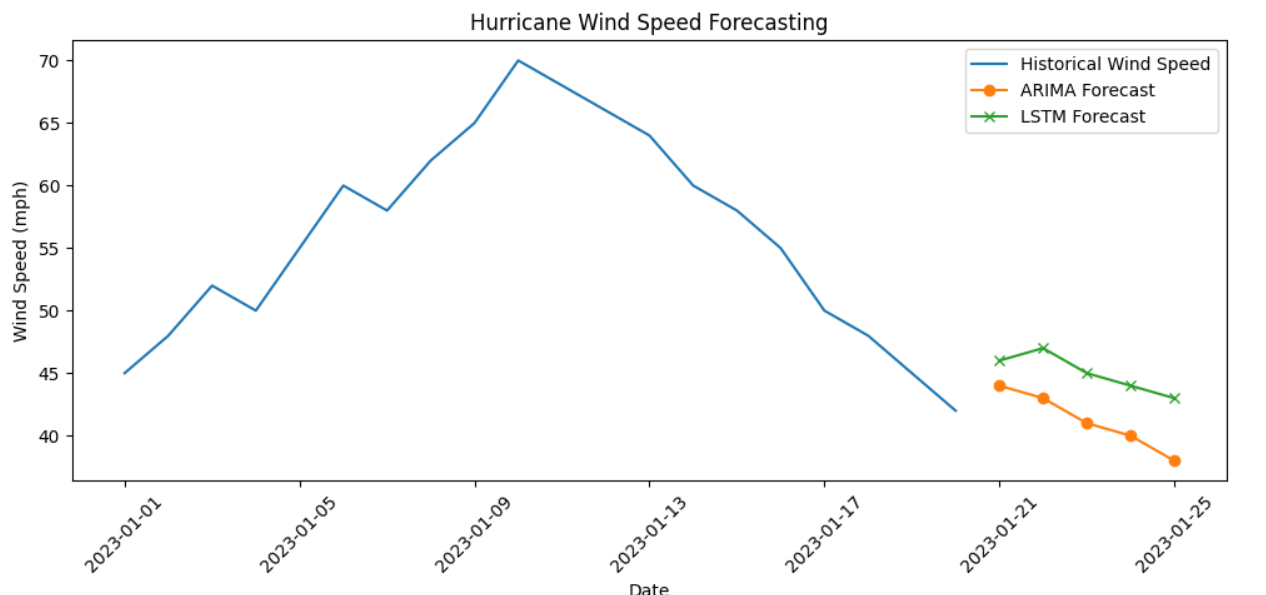
\includegraphics[width=1.0\textwidth]{../../BA25-02-Time-Series/report/Images/Output.png}
	\caption{Dummy Output Of Code}
	\label{fig:dummy_output}
\end{figure}

\subsection{Further Readings}

\begin{itemize}
	\item Box, G.E.P., Jenkins, G.M., Reinsel, G.C. (2015). \textit{Time Series Analysis: Forecasting and Control}. Wiley. \cite{BoxEtAl2015}
	\item Hochreiter, S., Schmidhuber, J. (1997). Long Short-Term Memory. \textit{Neural Computation}, 9(8), 1735–1780. \cite{HochreiterSchmidhuber1997}
	\item Hyndman, R.J., Athanasopoulos, G. (2021). \textit{Forecasting: Principles and Practice}. OTexts. \url{https://otexts.com/fpp3/}
	\item Emanuel, K. (2005). Increasing destructiveness of tropical cyclones over the past 30 years. \textit{Nature}, 436(7051), 686-688. \cite{Emanuel2005}
\end{itemize}
